\documentclass[11pt]{article}
\usepackage{mathtools}
\usepackage{mdframed}
\usepackage{fullpage}
\usepackage{amsfonts}
\usepackage{tikz}
\usepackage{fancyhdr}
\usepackage{lastpage}
\usepackage{graphicx}
\usepackage{pgfgantt}


%edit this for each class
\newcommand\name{John Collin Vincent}
\newcommand\classname{}
\newcommand\assignment{}

\graphicspath{{coms352/hw4/}}
\newcounter{excounter}
\setcounter{excounter}{1}
\newcommand\ques[2]{\vskip 1em  \noindent\textbf{\arabic{excounter}\addtocounter{excounter}{1}.} \emph{#1} \noindent#2}
\newenvironment{question}{\ques{}\begin{quote}}{\end{quote}}
\newenvironment{subquestion}[1]{#1) \begin{quote}}{\end{quote}}

\pagestyle{fancy}
\rfoot{\name, page \thepage/\pageref{LastPage}}
\cfoot{}
\rhead{}
\lhead{}
\renewcommand{\headrulewidth}{0pt}
\renewcommand{\footrulewidth}{0pt}
\DeclarePairedDelimiter\ceil{\lceil}{\rceil}
\DeclarePairedDelimiter\floor{\lfloor}{\rfloor}


\begin{document}


  {\bf \classname \hspace{1cm} \assignment\hfill \name}
  \vskip 2em


  \begin{subquestion}{1}
    they both end with 4 processes but the first program makes 6 prints to the terminal, 2 being duplicates from the loop.
    Also every once in a while when I run these programs the third process thats created claims that one of my systemd processes
    is its parent, when its parent should be the initial process. If you know why this happens please email me because I can't find
    and explination jvincent@iastate.edu.\\
    \center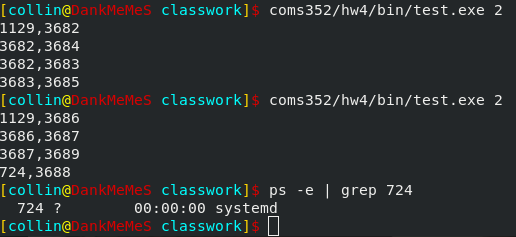
\includegraphics[width=.5\textwidth]{coms352/hw4/screenshot.png}
  \end{subquestion}

  \begin{subquestion}{6.16}
    \center FCFS\\
    \begin{ganttchart}[y unit title=0.4cm,
      y unit chart=0.5cm,
      vgrid,hgrid,
      title label anchor/.style={below=-1.6ex},
      title left shift=.05,
      title right shift=-.05,
      title height=1,
      bar/.style={fill=gray!50},
      incomplete/.style={fill=white},
      progress label text={},
      bar height=0.7,
      group right shift=0,
      group top shift=.6,
      group height=.3]{1}{20}
      %labels
      \gantttitlelist{0,...,19}{1}\\
      %tasks
      \ganttbar{$P_1$}{1}{2} \\
      \ganttbar{$P_2$}{3}{3} \\
      \ganttbar{$P_3$}{4}{11} \\
      \ganttbar{$P_4$}{12}{15} \\
      \ganttbar[progress=33]{$P_5$}{16}{20}
    \end{ganttchart}\\
    SJF\\
    \begin{ganttchart}[y unit title=0.4cm,
      y unit chart=0.5cm,
      vgrid,hgrid,
      title label anchor/.style={below=-1.6ex},
      title left shift=.05,
      title right shift=-.05,
      title height=1,
      bar/.style={fill=gray!50},
      incomplete/.style={fill=white},
      progress label text={},
      bar height=0.7,
      group right shift=0,
      group top shift=.6,
      group height=.3]{1}{20}
      %labels
      \gantttitlelist{0,...,19}{1}\\
      %tasks
      \ganttbar{$P_1$}{2}{3} \\
      \ganttbar{$P_2$}{1}{1} \\
      \ganttbar{$P_3$}{13}{20} \\
      \ganttbar{$P_4$}{4}{7} \\
      \ganttbar[progress=33]{$P_5$}{8}{12}
    \end{ganttchart}\\
    Nonpreemptive priority\\
    \begin{ganttchart}[y unit title=0.4cm,
      y unit chart=0.5cm,
      vgrid,hgrid,
      title label anchor/.style={below=-1.6ex},
      title left shift=.05,
      title right shift=-.05,
      title height=1,
      bar/.style={fill=gray!50},
      incomplete/.style={fill=white},
      progress label text={},
      bar height=0.7,
      group right shift=0,
      group top shift=.6,
      group height=.3]{1}{20}
      %labels
      \gantttitlelist{0,...,19}{1}\\
      %tasks
      \ganttbar{$P_1$}{14}{15} \\
      \ganttbar{$P_2$}{20}{20} \\
      \ganttbar{$P_3$}{1}{8} \\
      \ganttbar{$P_4$}{16}{19} \\
      \ganttbar{$P_5$}{9}{13}
    \end{ganttchart}\\\clearpage
    Round Robin\\
    \begin{ganttchart}[y unit title=0.4cm,
      y unit chart=0.5cm,
      vgrid,hgrid,
      title label anchor/.style={below=-1.6ex},
      title left shift=.05,
      title right shift=-.05,
      title height=1,
      bar/.style={fill=gray!50},
      incomplete/.style={fill=white},
      progress label text={},
      bar height=0.7,
      group right shift=0,
      group top shift=.6,
      group height=.3]{1}{20}
      %labels
      \gantttitlelist{0,...,19}{1}\\
      %tasks
      \ganttbar{$P_1$}{1}{2} \\
      \ganttbar{$P_2$}{3}{3} \\
      \ganttbar{$P_3$}{4}{5}\ganttbar{}{10}{11}\ganttbar{}{16}{17}\ganttbar{}{19}{20} \\
      \ganttbar{$P_4$}{6}{7} \ganttbar{}{12}{13}\\
      \ganttbar{$P_5$}{8}{9} \ganttbar{}{14}{15}\ganttbar{}{18}{18}
    \end{ganttchart}\\
    \raggedright
    \begin{subquestion}{b}
      \begin{center}
        FCFS\\
        $P_1 = 2, P_2 = 3, P_3 = 11, P_4 = 15, P_5 = 20$\\
        SJF\\
        $P_1 = 3, P_2 = 1, P_3 = 20, P_4 = 7, P_5 = 12$\\
        Nonpreemptive priority\\
        $P_1 = 15, P_2 = 20, P_3 = 8, P_4 = 19, P_5 = 13$\\
        Round Robin\\
        $P_1 = 2, P_2 = 3, P_3 = 20, P_4 = 13, P_5 = 18$\\
      \end{center}
    \end{subquestion}
    \begin{subquestion}{c}
      \begin{center}
        FCFS\\
        $P_1 = 0, P_2 = 2, P_3 = 3, P_4 = 11, P_5 = 15$\\
        SJF\\
        $P_1 = 1, P_2 = 0, P_3 = 12, P_4 = 3, P_5 = 7$\\
        Nonpreemptive priority\\
        $P_1 = 13, P_2 = 19, P_3 = 0, P_4 = 15, P_5 = 8$\\
        Round Robin\\
        $P_1 = 0, P_2 = 2, P_3 = 12, P_4 = 9, P_5 = 13$\\
      \end{center}
    \end{subquestion}
    \begin{subquestion}{c}
      \begin{align*}
        FCFS &= \frac{0+2+3+11+15}{5} &= 6.2\\
        SJF &= \frac{1+0+12+3+7}{5} &= 4.6\\
        NonPreemptive &= \frac{13+19+0+15+8}{5} &= 11\\
        Round Robin &= \frac{0+2+12+9+13}{5} &= 7.2\\
      \end{align*}\\
      shortest job first has the lowest average wait time.
    \end{subquestion}
  \end{subquestion}

  \clearpage

  \begin{subquestion}{6.19}
    Shortest job first can cause starvation if small jobs keep getting added to the queue, the longer jobs will
    never execute.\\
    Priority can cause starvation because if high priority jobs keep getting scheduled the low priority jobs will never be executed
  \end{subquestion}

  \begin{subquestion}{6.22}
    They could limit the number of other user processes, and keep the process in the highest priority queue possible.
  \end{subquestion}


\end{document}
